\documentclass[thesis.tex]{subfiles}
\renewcommand\_{\textunderscore\allowbreak}

\begin{document}


\chapter{Object Definitions and Event Selection}
\label{cap:eventSelection}

\section{Definition of Particle Identification Variables}
A description of variables used for particle identification (ID) and selection is given here:

\noindent \textbf{Calorimeter shower shape variables}:
\begin{itemize}
	\item $R_9$: sum of energy of the $3\times3$ crystals centred on the most energetic crystal in the supercluster divided by that of $5\times5$ crystals. 
	\item \Sigmaieie: lateral width of the electromagnetic shower in $\eta$ direction. \\
		It is calculated as: $\Sigmaieie = \sqrt{\sum_i^{5\times5}[(\eta_i^{\text{cryst.in cluster}}\times 0.0175 + \eta^{\text{seed cryst.}} - \bar{\eta}_{5\times5})^2 \times w_i/{\sum_i^{5\times5}w_i}}]$, where $w_i = 4.2+ln\frac{E_i}{E_{5\times5}}$.
\end{itemize}
\noindent \textbf{Isolation variables}:
\begin{itemize}
	\item $\HoverE$: ratio of energy deposited in the HCAL tower behind the ECAL supercluster and energy of the supercluster.
	\item PF charged isolation \ChIso: transverse energy sum of all PF charged hadrons falling inside a cone of size \DeltaR = 0.3 around the candidate particle. Contributions from pileup are estimated by multiplying the median density of pileup contamination ($\rho$) per event with the effective area of the cone. The pileup contributions are then subtracted from the isolaiton. This is the so-called ``$\rho$ correction'' method. 
	\item PF neutral isolation \NeuIso:  transverse energy sum of all PF neutral hadrons falling inside a cone of size \DeltaR = 0.3 around the candidate particle. $\rho$ correction is applied to mitigate the pileup effect. 
	\item PF photon isolation \PhoIso: transverse energy sum of all PF photons reconstructed inside a cone of size \DeltaR = 0.3 around the candidate particle. Footprint of the candidate itself has been removed to avoid double counting. $\rho$ correction is applied to mitigate the pileup effect.
\end{itemize}

\noindent \textbf{Electron ID variables}:
\begin{itemize}
	\item $|\Delta\eta_{in}| = |\eta_{SC} - \eta_{in}^{\text{extrap}}|$: the distance between SC energy-weighted $\eta$ ($\eta_{SC}$) and the track $\eta$ extrapolated from the tracker to the ECAL ($\eta_{in}^{\text{extrap}}$).
	\item $|\Delta\phi_{in}| = |\phi_{SC} - \phi_{in}^{\text{extrap}}|$: the distance between SC and track extrapolated position in $\phi$
	\item $|\frac{1}{E} - \frac{1}{p}|$: the difference between the SC energy (E) and track momentum ($p$).  
\end{itemize}

\noindent \textbf{Muon ID variables}:
\begin{itemize}
	\item $\chi^2/d.o.f.$: $\chi^2$ of the track normalized to the degree of freedom in fitting 
	\item $\chi^2$ of the kick finder: the $\chi^2$ between the inward and outward states of a track in each layer is calculated to look for kicks, and the largest $\chi^2$ per track is used as the $\chi^2$ for kick finder.
	\item $\Dxy$: transverse impact parameter relative to the beam-spot position
	\item $\Dz$: longitudinal impact parameter relative to the beam-spot position 
\end{itemize}


\section{Photon}
\label{sec:photonID}
The default format of the photons in miniAOD datasets is ``slimmedPhotons'', which keeps high level physics objects. 
$e/\gamma$ energy scales, which are described in \ref{sec:reco-photon}, are applied to the photons to optimize the energy reconstruction and resolution. 

Photons with $p_{T} >$ 35 GeV reconstructed in the ECAL barrel ($|\eta| <$ 1.4442) region are used. 
They are required to match the trigger objects of the HLT within $\Delta R <$ 0.3. 
To ensure that photon candidates pass the $R_9$ filter in the $e\gamma$ trigger, the photons are in addition required to have $R_9 <$ 0.5.
Out of such preselected photons, those fulfilling a set of ID criteria are selected.
The selection criteria usually requires the ID variables of a particle to either above some thresholds or below certain upper bounds, which are called ``cuts''. 
Photons in this search are selected using the loose working point ID, which includes the following cuts: 
\begin{center}
\begin{itemize}
\item H/E $<$ 0.0597
\item $\sigma_{i\eta i\eta} <$ 0.01031 
\item Iso$_h^\pm <$ 1.295
\item Iso$_h^0 < 10.910 +0.0148 \cdot p_{T} + 0.000017 \cdot p^2_{T}$
\item Iso$_{pho} < 3.630+0.0047 \cdot p_{T}$
\end{itemize}
\end{center}

To suppress the $e\rightarrow\gamma$ fake objects, candidate photons are required to not be associated with a pixel track seed. 
In addition, a photon is rejected if an electron is close to it within $\Delta R <$ 0.02. 
Such a veto help remove the very rare cases where the ECAL clusters fail to match pixel seeds but electrons still get reconstructed by ECAL-driven tracking algorithm.

The identification and pixel veto efficiencies are measured for both data and simulation by the CMS EGM group and are given in ~\cite{EGM:leptonScale}. The data-to-simulation efficiency scale factors (ESF) are applied on MC samples to correct the simulation response. Fig. \ref{fig:photonsf} shows the 2D map of photon scale factors along with the uncertainty of each $\eta-p_T$ bin.

\begin{figure*}[hbtp]
	\centering
	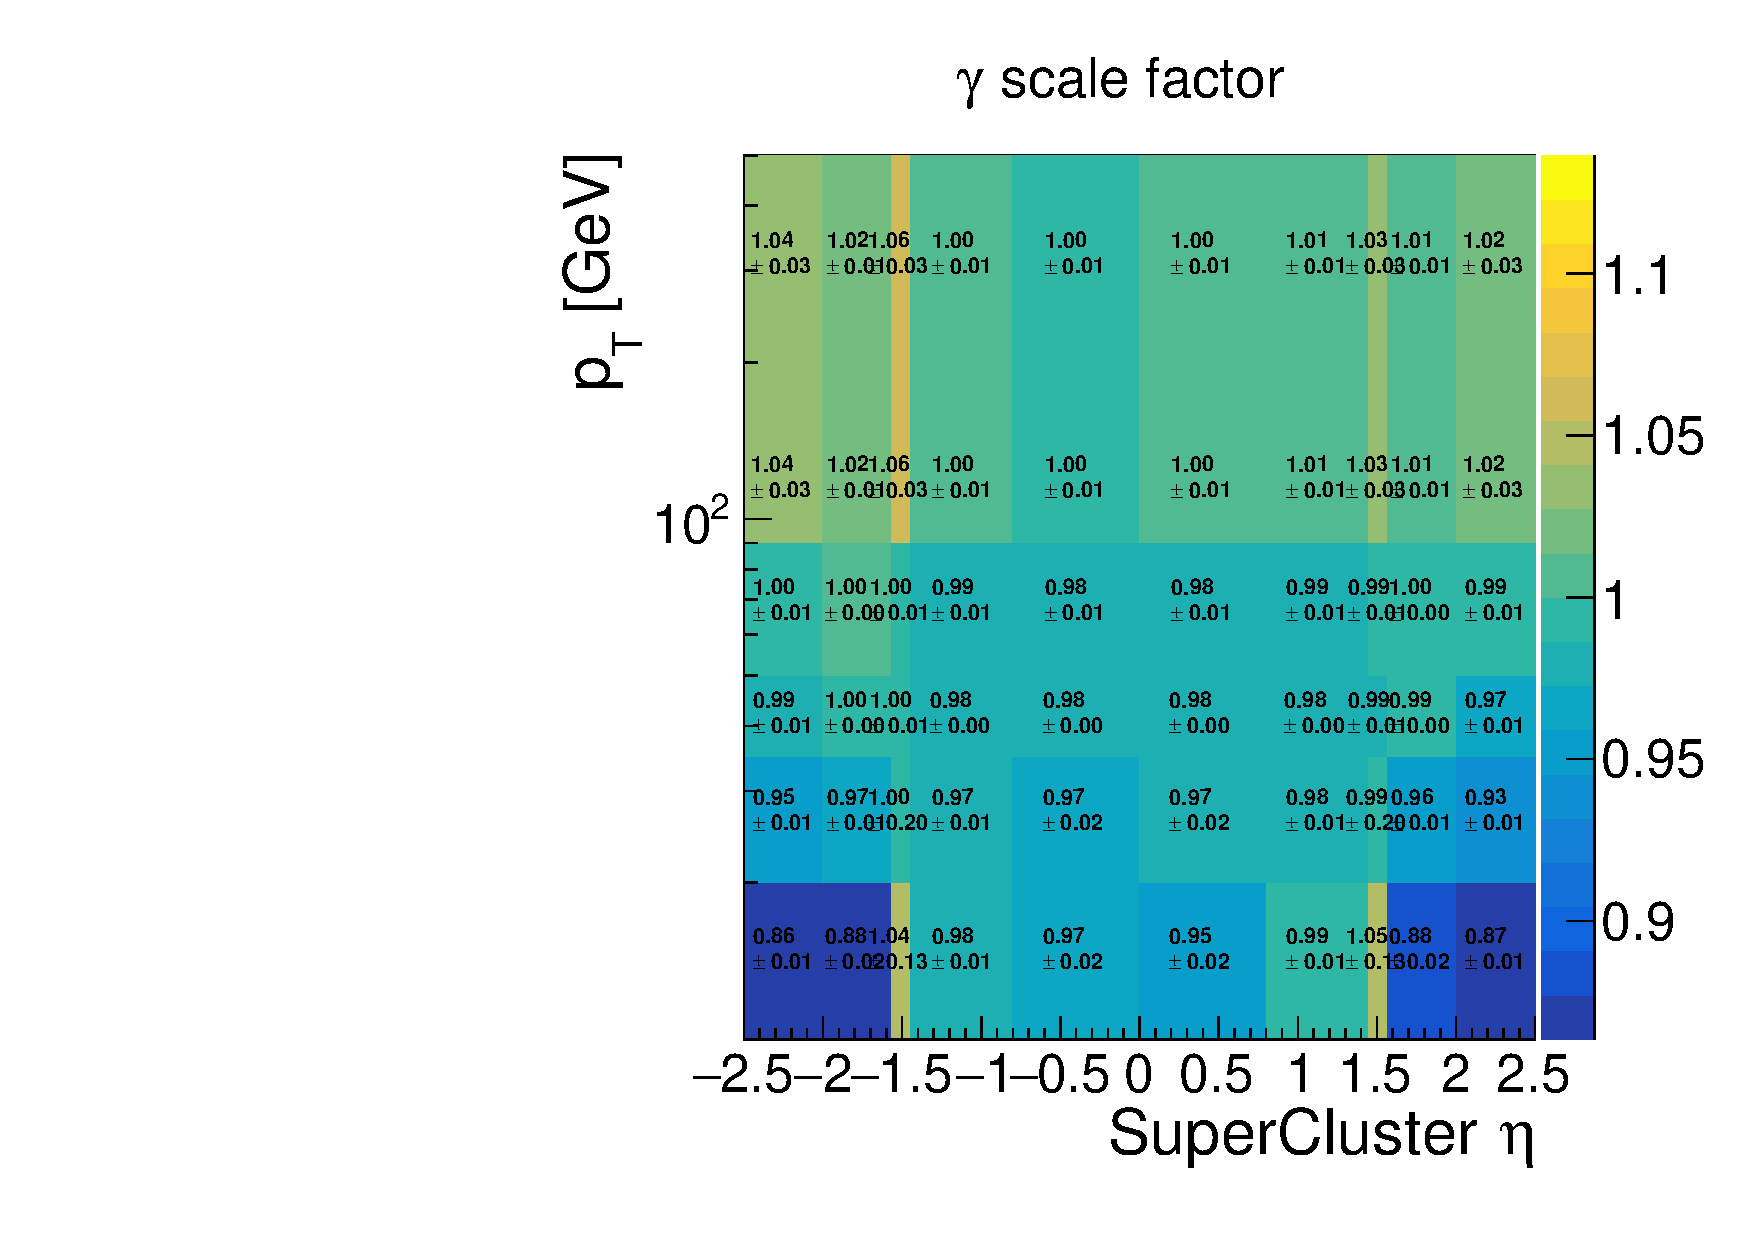
\includegraphics[width=0.5\textwidth]{plot/SF_Photon.pdf}
	\caption{data-to-simulation scale factors for photons.}
	\label{fig:photonsf}
\end{figure*}


\section{Electron}
\label{sec:electronID} 
Electrons with  $p_{T} >$ 25 GeV reconstructed in the pesudorapidity range $|\eta| <$ 2.5 are used. To ensure a good acceptance efficiency, objects falling in the barrel-endcap region 1.442 $< |\eta| <$ 1.56 are rejected. 

Electrons passing the kinematic cuts are required to match the sub-leading leg of the di-photon trigger. 
To mimic the $R_9$ filters in trigger, a $R_9 <$ 0.5(0.8) preselection cut is applied on the electrons in EB(EE). 
Candidate electrons are then identified using cut-based medium working point ID, including the following selections:

\begin{center}
\begin{itemize}
\item $\sigma_{i\eta i\eta} <$ 0.00998(EB), 0.0298(EE)
\item $\Delta\eta_{in} <$ 0.00311(EB), 0.00609(EE)
\item $\Delta\phi_{in} <$ 0.103(EB), 0.045(EE)
\item $\HoverE$ $<$ 0.253(EB), 0.0878(EE)
\item $|\frac{1}{E} - \frac{1}{p}| <$ 0.0129
\item At most one expected missing hit in inner tracker layers
\item Pass conversion veto
\end{itemize}
\end{center}

The conversion veto is applied to reject the electrons that arise from conversions of photons.
When photon conversions happen inside the tracker, the tracks of the resulting electrons are more likely to begin later than prompt electrons, and missing hits are therefore present in the first few layers of the inner tracker. 
In addition, conversions are identified by fitting track pairs to a common vertex and searching for nearby partner tracks.
The conversion algorithm combines all these methods to veto the photon conversions.

The relative isolation cut is removed from the medium ID selections. 
Instead, we use the mini-Isolation~\cite{CMS:Isolation}, which is defined as the ratio of the energy sum in a cone to the $p_T$ of the electron.
The cone size is $p_T$-dependent: R = 10 GeV/min(max($p_T(e)$, 50 GeV), 200 GeV), resulting in a radii of 0.05 for low-$p_T$ electrons and 0.2 for high-$p_T$ ones. 
The use of mini-Isolation ensures a good acceptance of lepton even in Lorentz-boosted topologies.
In this analysis, we required the mini-Isolation of the electron to be smaller than 0.1. 

The efficiencies of the electron identification and mini-Isolation filters are measured by EGM group and are given in \cite{EGM:leptonScale}. Fig. \ref{fig:elesf} shows the data-to-simulation ESF of the electron ID and mini-Isolation. 

\begin{figure*}[hbtp]
	\centering
	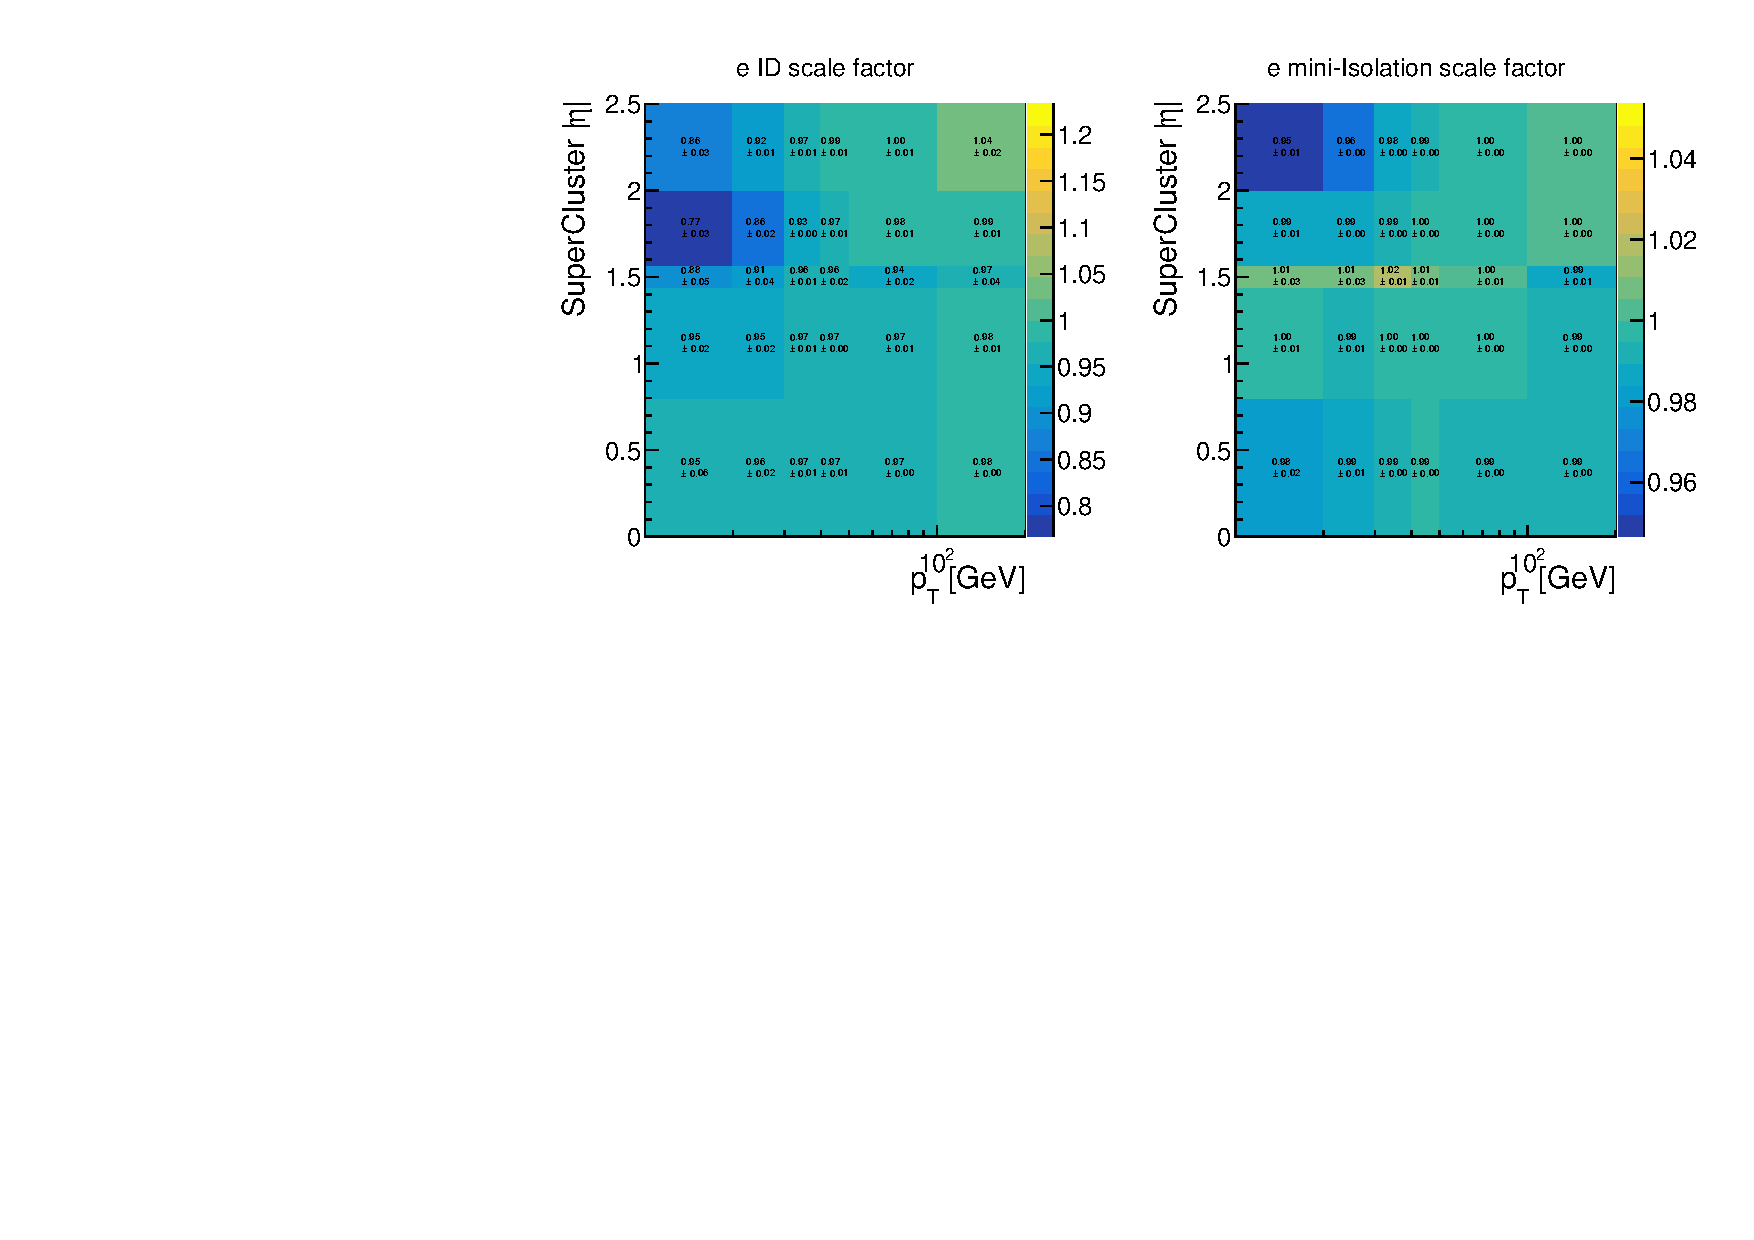
\includegraphics[width=0.99\textwidth]{plot/SF_Ele.pdf}
	\caption{data-to-simulation scale factors for electrons.}
	\label{fig:elesf}
\end{figure*}

\section{Muon}
Muons with $p_{T} >$ 25 GeV in the pesudorapidity range $|\eta| <$ 2.4 are used. 
A matching to the trigger leg is required for a muon to enter the candidate collection. 
The muon is identified using the standard medium ID, defined as:

\begin{center}
\begin{itemize}
\item Is PF muon
\item Is also reconstructed as a global-muon or as an tracker-muon
\item Fraction of valid tracker hits $>$ 0.8
\item Either satisfies the good global muon criteria:
	\begin{itemize}
		\item is global muon
		\item normalized $\chi^2$ of the global track is less than 3
		\item $\chi^2$ of the position of the standalone muon and associated tracker tracks is less than 12
		\item $\chi^2$ of the kick finder is less than 20
		\item segment compatibility between the tracker tracks and muon chambers is greater than 0.303
	\end{itemize} 
	or has a segment compatibility greater than 0.451
\end{itemize}
\end{center}

The Muon is in addition required to pass the impact parameter and isolation cuts:
\begin{center}
\begin{itemize}
\item $\Dxy <$ 0.05 cm, $\Dz <$ 0.1 cm.
\item mini-Isolation $<$ 0.2.
\end{itemize}
\end{center}

Both the identification efficiency and isolation efficiency are measured by CMS SUSY group and are given in \cite{EGM:leptonScale}. Fig. \ref{fig:muonsf} shows the ESF used for muon data-to-simulation corrections.

\begin{figure*}[hbtp]
	\centering
	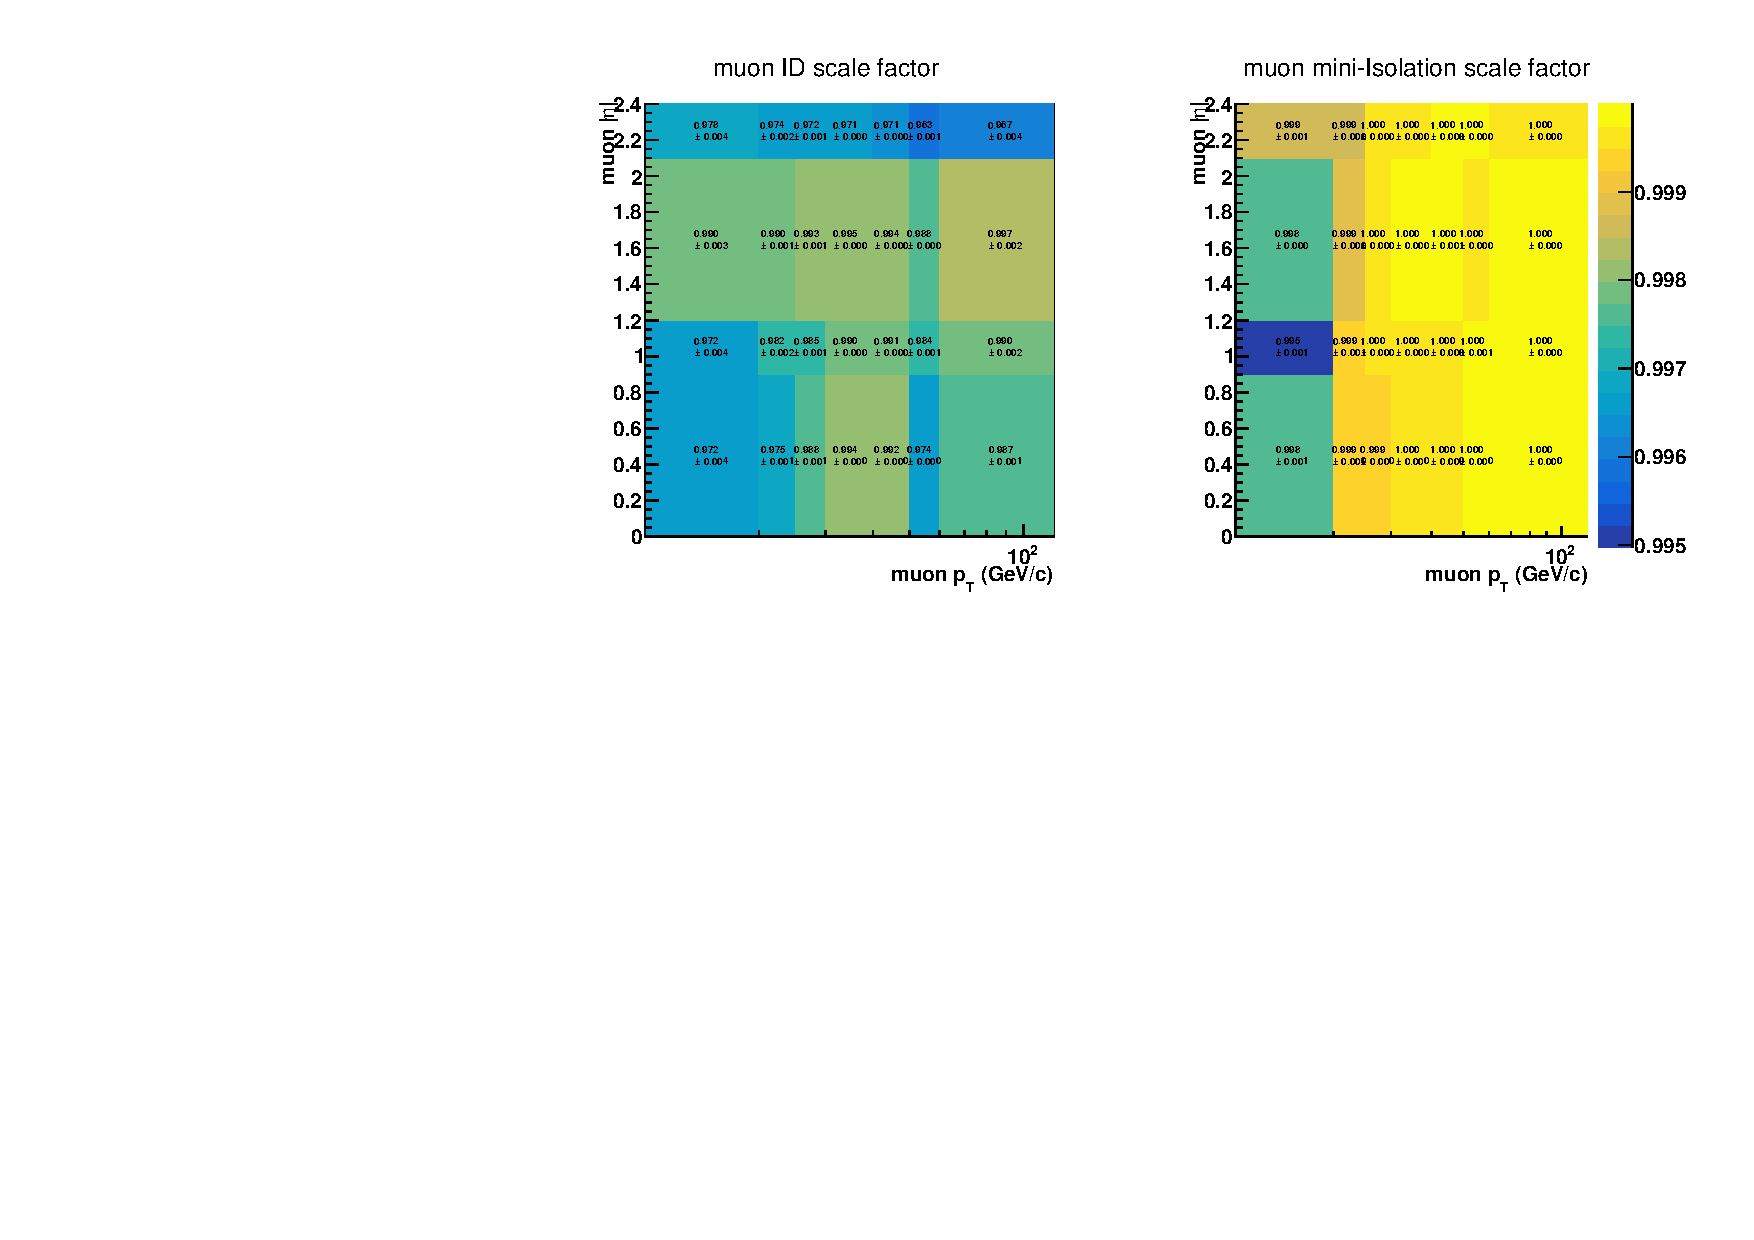
\includegraphics[width=0.99\textwidth]{plot/SF_Muon.pdf}
	\caption{data-to-simulation scale factors for muons.}
	\label{fig:muonsf}
\end{figure*}

If more than one candidate object are identified in an event, the one with the highest $p_{T}$ is used.

\section{Jet and HT}
\label{sec:jetID}
ak4PFJets jets, which are reconstructed using the anti-$k_T$ algorithm with a radii of 0.4, are used in this search.
Jets with $p_T >$ 30 GeV and $|\eta| <$ 2.5 are selected. 
The raw energy of the jets are first corrected to take account the contributions from pileup.
Then, jet energy corrections \cite{CMS:JES} derived from the simulation are applied to scale the reconstructed energy.
Finally, the jet energy is further corrected using di-jet events. 

To avoid double counting, jets that overlap with photon or lepton candidate with $\DeltaR <$ 0.4 are not considered.
The cone size of 0.4 is chosen because the ak4 algorithm uses R = 0.4 to cluster the jets.  

$H_T$ is a variable that quantifies the hadronic activity of an event. 
It is defined as the scale sum of $p_T$ of all selected jets, as:
	\begin{equation*}
		 H_T = \sum_i^{N_{jets}}|p_{T,i}|
	\end{equation*}
Events from electroweak production usually have small $H_T$, whereas those from hadronic production tend to have larger $H_T$. 


\section{Missing Transverse Momentum}
The type-1 corrections is applied to the raw MET. This correction propagate the jet energy corrections to MET.

A set of MET Filters recommended by the JetMET group are applied to clean events with large fake MET, such as detector noise, cosmic rays and beam halos. Events are rejected if they fail the following filters:
\begin{center}
\begin{itemize}
\item primry vetex filter:\\
		At least one good vertex is required to be present in each event. A vertex is considered to be good if it has at least 5 degrees of freedom and its distance from the interaction point is less than 24 cm in z direction and 2cm in the x-y plane. 
\item beam halo filter
\item HBHE noise filter
\item HBHEiso noise filter
\item ECAL TP filter
\item Bad PF Muon Filter
\item Bad Charged hadron filter
\item EE badSC noise filter
\item badMuons flag
\item duplicateMuons flag
\end{itemize}
\end{center}

\section{Photon FSR}
  Photons emitted in vector boson (W or Z ) decays or radiated off the leptons can be energetic and isolated. Such events are called final state radiation (FSR) and can mimic the SUSY signals if large MET is also present. Simulation shows that the separation between the photon and the lepton is typically smaller in final states events (FSR) than in SUSY signal events, as shown in Figure [to be produced]. Therefore, three additional cuts are designed to suppress the FSR contributions:
\begin{itemize}
\item The candidate photon must be well separated from the candidate electron by $\Delta R >$ 0.8
\item No leptons are reconstructed close to the candidate photon within $\Delta R <$ 0.3
\item In the $e\gamma$ channel, $M_{e\gamma} > M_Z + 10 $GeV 
\end{itemize}

The last cut is applied on top of the 90 GeV invariant mass filter of the $e\gamma$ HLT to further reject $Z\rightarrow ee$ events, where one of the electrons is misidentified as a photon.

\end{document}
